\documentclass[11pt]{article}	% Everything after % in a line is comment

% Some commonly used packages. You can add more packages if you need
\usepackage[margin=1in]{geometry}
\usepackage{amsmath,amssymb,amsthm}
\usepackage{graphicx}
\usepackage{url}
\usepackage{float}

\title{Team Project Outline in LaTeX Template}
\author{Ratislav Krylov \and Caleb Lewis} 
\date{} % Fill in actual date, or comment this line to show current date.

\begin{document}
\maketitle

\begin{abstract}
Many useful differential equations either cannot be solved analytically or do not have analytical solutions. 
In this paper we explore the power of different numerical analysis methods by implementing
them in Python.
Methods such as Runge-Kutta Four and Euler have different computational cost, so in order
to keep comparison fair the step size is adjusted so that both methods have similar cost.
The errors of both methods are plotted and compared to see which one performs better on
example problems. One of the surprising findings is that Runge-Kutta Two outperformed 
Modified Euler method, even though both of them have similar computational cost and order of 
local truncation error. We also discovered that Predictor-Corrector method outperforms RK4 in
all examples as well. 
\end{abstract}

\section{Introduction}
%A section briefly introduces the background and purpose of this paper.
This is an exploratory report meant to be our proving and playing ground where we explore
methods learned in Numerical Analysis II class. In the class, we have closely covered Euler,
Modified Euler, Midpoint Method, Runge-Kutta 4, Adams-Bashforth 4-step explicit method,
and Adams 4th-order Predictor corrector method, as well as some other methods that are not
covered in this paper. While we have done some review of the proofs for Euler method, this 
paper mainly focuses on numerical exploration of these methods. We implement different techniques using python and compare them on the set of 3 textbook problems. Visual plots of errors are made 
to make it easier to see how they each compare to each other. To measure up methods fairly, we take
things such as computational costs and memory costs into account.

\section{Methods in this study}
%Show the methods that you're studying in this term paper.
%For example, you can write some subsections as follows to 
%explain the difference scheme of each method, its complexity, local truncation error, etc.
All numerical methods that we have covered so far have a similar theme. With differential equations and initial values, we are able to find slopes of the curves and apply a sort of linearization on them to find an approximation for the next value. While the complexity of some of these numerical methods has increased, this basic premise seems to have remained. 

\subsection{Euler's Method}
Euler's method is one of the oldest numerical methods with intuitive rules. Given IVP:
(1) calculate the slope of the line 
$$y\prime = f(t, y) \hspace{0.15cm} for \hspace{0.15cm} t \in [a, b] \hspace{0.15cm} and \hspace{0.15cm} y(a) = \alpha $$ 
We can divide the interval into $N$ equal segments. Then Euler's method on this IVP is: 
$$w_0 = \alpha $$
$$w_{i+1} = w_i + hf(t_i, w_i)$$
Where $i = 0,1,..., N-1$ and $h = \frac{b-a}{N}$. 

Euler's method local truncation error is: 
$$|\tau _{i+h}(h) = \frac{hM}{2} = O(h).$$

Making it change linearly with step-size with the computational cost of one evaluation of $f(t, y)$ per step. 

\subsection{Modified Euler's Method}
Modified Euler's method is a take on the original idea of Euler's method that uses two function evaluations:
$$w_0 = \alpha $$
$$w_{i+1} = w_i + \frac{h}{2}(f(t_i,w_i) + f(t_{i+1}, w_i + hf(t_i,w_i)))$$
It has $O(h^2)$ local truncation error. 


\subsection{Runge-Kutta method}
%This is a subsection about RK2 and RK4 methods.
Runge-Kutta methods are a family of methods that see a big boost in comparison to Euler's method. One of them is RK2 with the following scheme:
$$w_0 = \alpha $$
$$w_{i+1} = w_i + hf(t_i + \frac{h}{2}, w_i + \frac{h}{2}f(t_i, w_i))$$
It evaluates the function twice and has a local truncation error of order $O(h^2)$.

The most cost-effective Runge-Kutta method is one with 4-th order local truncation error, commonly called RK4. It has the following scheme:
%include description of what each evaluation accomplishes and just a general intuitiveness of each method
$$w_0 = \alpha $$
$$k_1 = f(t_i, w_i)$$
$$k_2 = f(t_i + \frac{h}{2}, w_i + \frac{h}{2}k_1)$$
$$k_3 = f(t_i + \frac{h}{2}, w_i + \frac{h}{2}k_2)$$
$$k_4 = f(t_{i+1}, w_i + hk_3)$$
$$w_{i+1} = w_i + \frac{h}{6}(k_1 + 2k_2 + 2k_3 + k_4)$$

As can be seen, each step requires four evaluations. But the exponential increase in order of 
local truncation error makes it a quite worthy computational investment. 

\subsection{Adams-Bashforth Four-step explicit method}
This method is of the family of multistep methods. Multistep methods rely not only on one previous data point, but on multiple older evaluations. They require storage of previous data points to use for evaluation of next one, but since the previous data points are stored, they normally only require a single evaluation of function $f(t_i,w_i)$. Adams-Bashforth Four Step explicit method uses four previous data points to evaluate the next one. Its scheme is:
$$w_0 = \alpha , \hspace{1cm} w_1 = \alpha _1, \hspace{1cm} w_2 = \alpha _2, \hspace{1cm} w_3 = \alpha _3$$
$$w_{i+1} = w_i + \frac{h}{24}(55f(t_i,w_i) - 59f(t_{i-1}, w_{i-1}) + 37f(t_{i-2}, w_{i-2}) - 9f(t_{i-3}, w_{i-3}))$$
And local truncation error is: $\tau _{i+1}(h) = \frac{251}{720}y^{(5)}(\mu _i)h^4$

\subsection{Predictor-Corrector method}
Predictor-Corrector methods utilize the scheme of multistep implicit evaluations. Multistep implicit methods such as Adams-Moulton 3-step, predict the next value based on the next value. 
Predictor-Corrector methods utilize this quirk by first predicting the value using some explicit 
method of similar order and then correcting it with the implicit method. Example we explore here is
the Adams 4th-order Predictor-Corrector method. Since implicit and explicit methods rely on the same data points, the additional correction with implicit method does not require much more
resources. Given $w_0, w_1, w_2, w_3$ here are its steps: 
$$w_{i+1,p} = w_i + \frac{h}{24}(55f(t_i,w_i) - 59f(t_{i-1}, w_{i-1}) + 37f(t_{i-2}, w_{i-2}) - 9f(t_{i-3}, w_{i-3}))$$
$$w_{i+1} = w_i + \frac{h}{24}(9f(t_{i+1}, w_{i+1, p}) + 19f(t_i, w_i) - 5f(t_{i-1}, w_{i-1} + f(t_{i-2}, w_{i-2}))$$
Since both implicit and explicit methods have error of order $O(h^4)$ Adams Predictor-Corrector local truncation error is of that same order as well. 


%We consider the Adams 4th-order Predictor-Corrector method
%which uses the Adams-Bashforth 4-step explicit method for prediction and Adams-Moulton 3-step implicit
%method for correction. With initial value $w_0=\alpha$, suppose we first generate $w_1,w_2,w_3$
%using RK4 method. Then for $i=3,4,\dots,N-1$:
%\begin{itemize}
%\item Use Adams-Bashforth 4-step explicit method to get a predictor $w_{i+1,p}$:
%\begin{equation}\label{eq:p-step}
%w_{i+1,p} = w_i + \frac{h}{24} [ 55 f(t_i, w_i) - 59 f(t_{i-1}, w_{i-1}) + 37 f(t_{i-2}, w_{i-2}) - 9 %f(t_{i-3},w_{i-3}) ]
%\end{equation}
%\item Use Adams-Moulton 3-step implicit method to get a corrector $w_{i+1}$:
%\begin{equation}\label{eq:c-step}
%w_{i+1} = w_i + \frac{h}{24} [ 9 f(t_{i+1},w_{i+1,p}) + 19 f(t_i, w_i) - 5 f(t_{i-1}, w_{i-1}) + %f(t_{i-2}, w_{i-2}) ]
%\end{equation}
%\end{itemize}
%The output of iteration $i$ is $w_{i+1}$ after prediction step \eqref{eq:p-step} and correction step \eqref{eq:c-step}.

\section{Numerical experiments}
In the following sections are the plots of methods 

\newpage
\subsection{Example 1}
\begin{figure}[H]
\centering
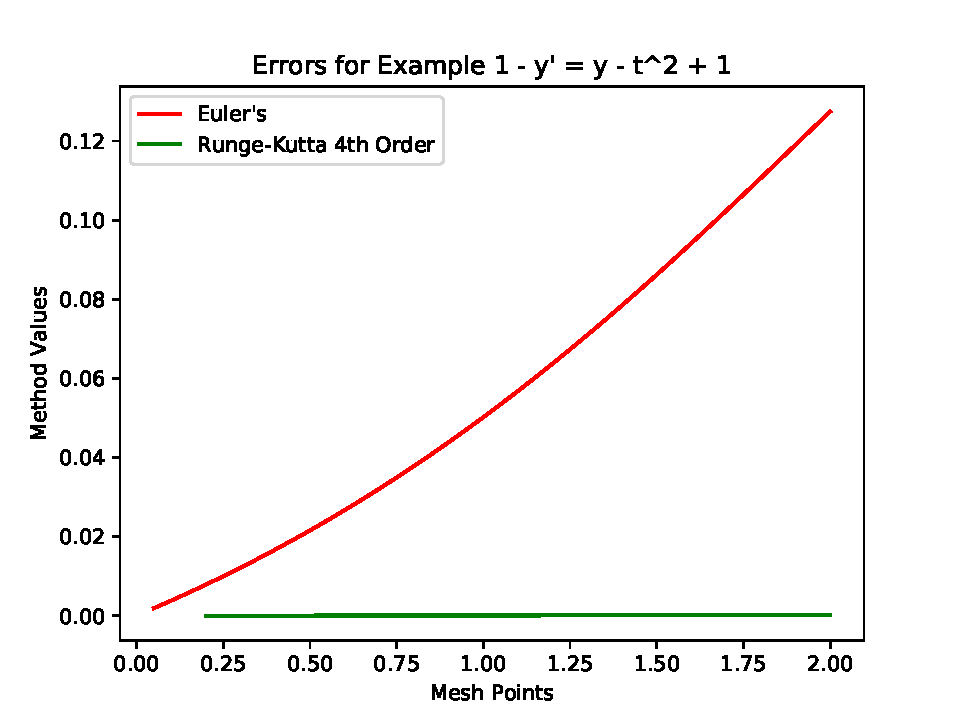
\includegraphics[width=.45\textwidth]{euler_rk4_1}
\caption{Accuracy of Euler vs RK4 when the former has four times smaller step-size. Ex. 1}
\label{fig:euler_rk4_1}
\end{figure}

\begin{figure}[H]
\centering
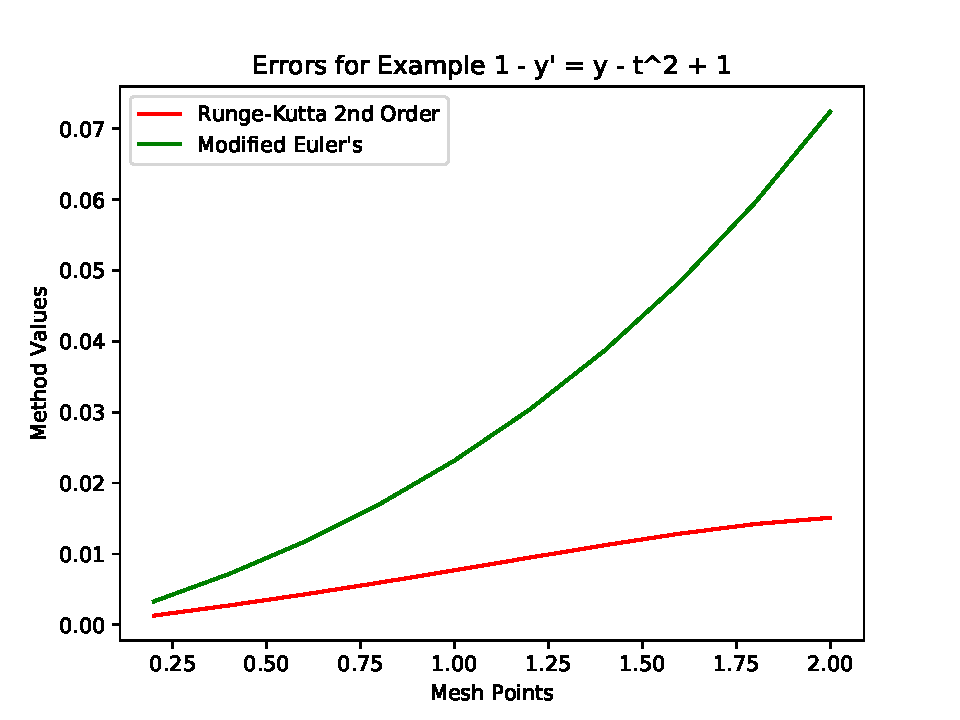
\includegraphics[width=.45\textwidth]{rk2_meuler_1}
\caption{Accuracy of RK2 vs. Modified Euler's method. Ex. 1}
\label{fig:rk2_meuler_1}
\end{figure}

\begin{figure}[H]
\centering
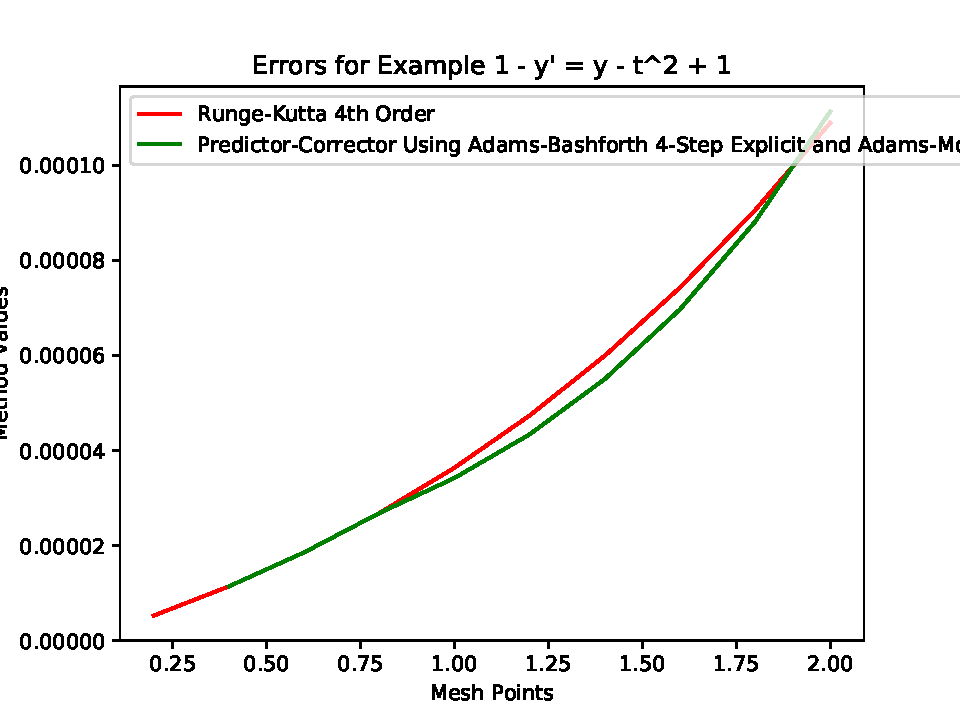
\includegraphics[width=.45\textwidth]{rk4_predictor_1}
\caption{Accuracy of RK4 vs  Adams 4th-order Predictor-Corrector method. Ex. 1}
\label{fig:rk4_predictor_1}
\end{figure}

\vfill
\clearpage

\newpage
\subsection{Example 2}

\begin{figure}[H]
\centering
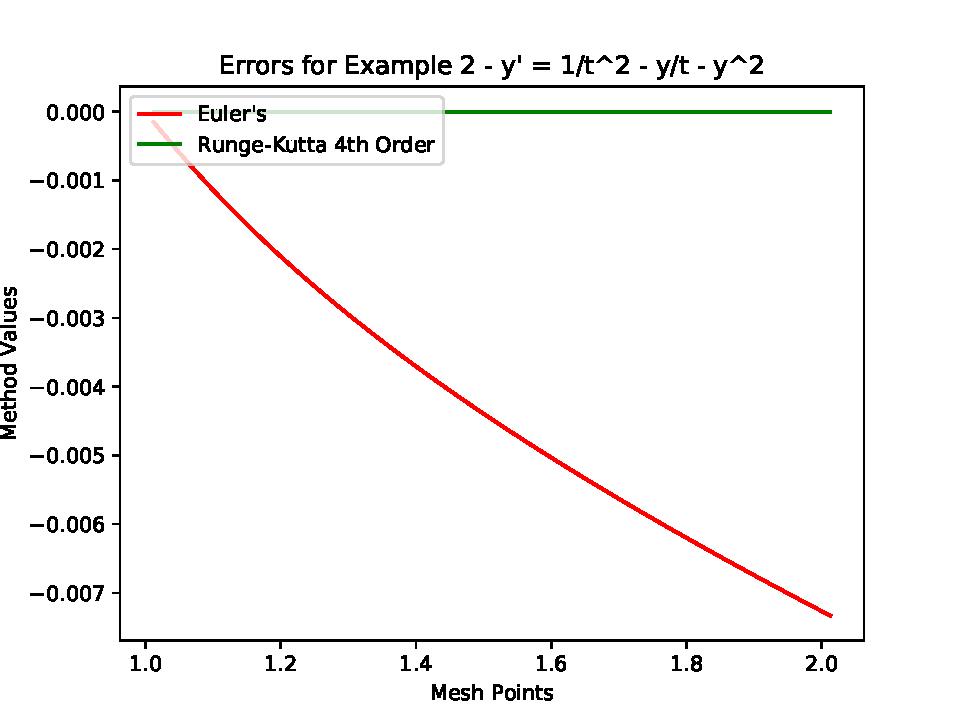
\includegraphics[width=.4\textwidth]{euler_rk4_2}
\caption{Accuracy of Euler vs. RK4 when the former has four times smaller step-size. Ex. 2}
\label{fig:euler_rk4_2}
\end{figure}

\begin{figure}[H]
\centering
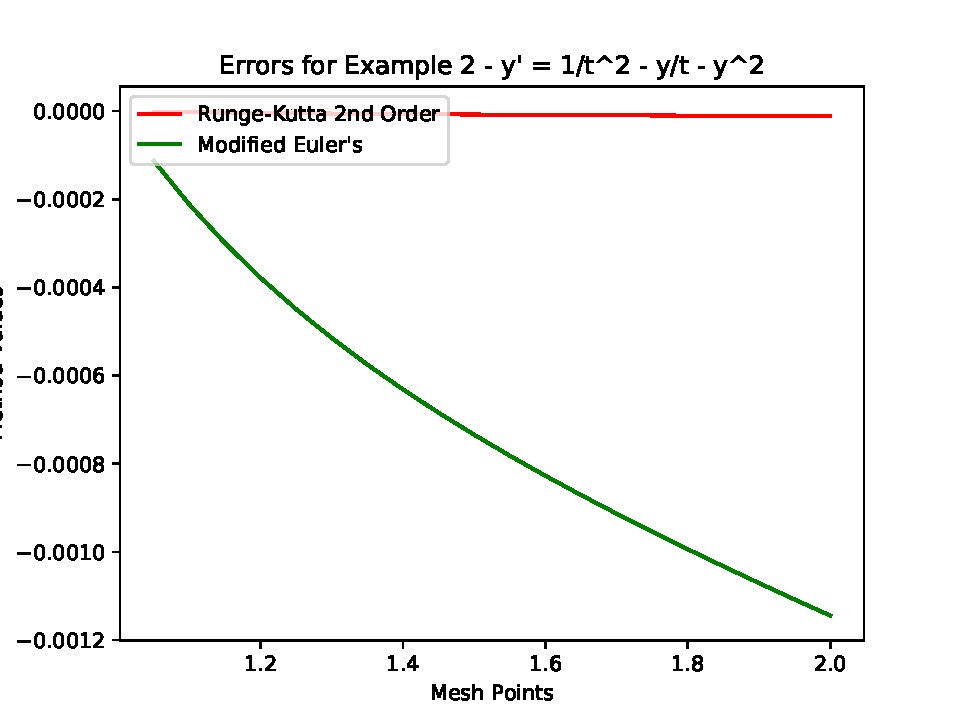
\includegraphics[width=.4\textwidth]{rk2_meuler_2}
\caption{Accuracy of RK2 vs. Modified Euler's method. Ex. 2}
\label{fig:rk2_meuler_2}
\end{figure}

\begin{figure}[H]
\centering
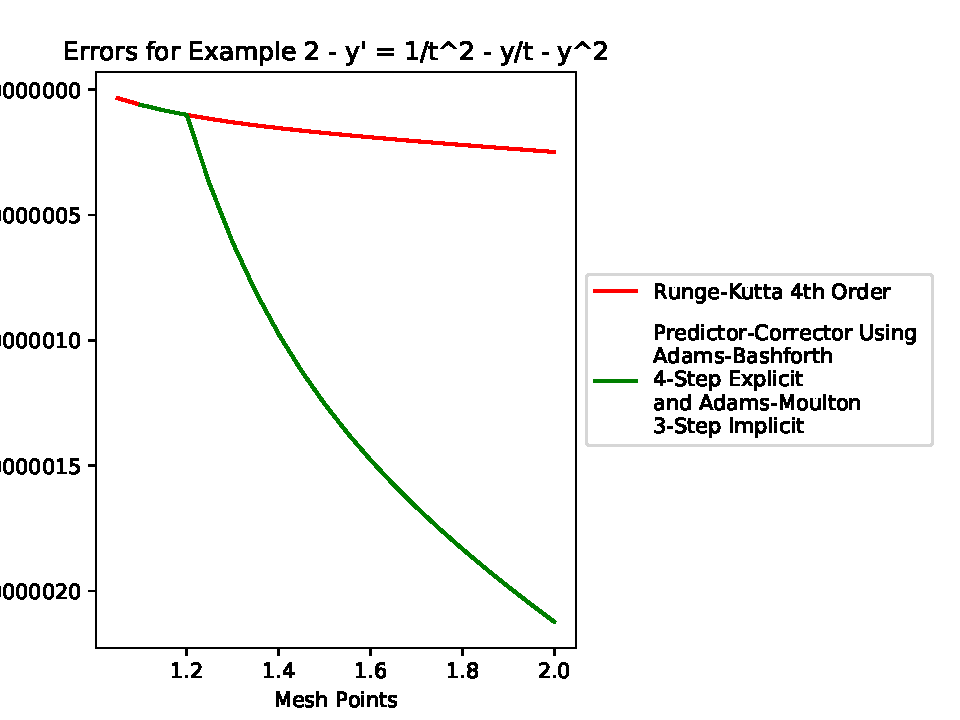
\includegraphics[width=.4\textwidth]{rk4_predictor_2}
\caption{Accuracy of RK4 vs. Adams 4th-order Predictor-Corrector method. Ex. 2}
\label{fig:rk4_predictor_2}
\end{figure}
\clearpage
\newpage
\subsection{Example 3}

%You will need to demonstrate the performance
%of the methods on several (ideally 3 to 5) example IVPs (of your own choice).
%You can choose some problems from textbook, but make sure that you 
%explicitly state what the problem you chose for each test.

%To show the performance, it is often better to use figures
%rather than tables (unless there are very few numbers to show). 
%For example, you 
%can show the result of RK4
%using Figure \ref{fig:rk4_example}. If you have multiple results, you can plot each
%with a curve (in different color/line-style/marker type) in the plot. If they are too close, you can %consider to 
%plot $|w_i-y_i|$, the error of estimate $w_i$ to true solution $y_i=y(t_i)$,
%instead of actual $y_i$ and $w_i$. This way, you can see which methods have lower errors (higher %accuracy).

\begin{figure}[H]
\centering
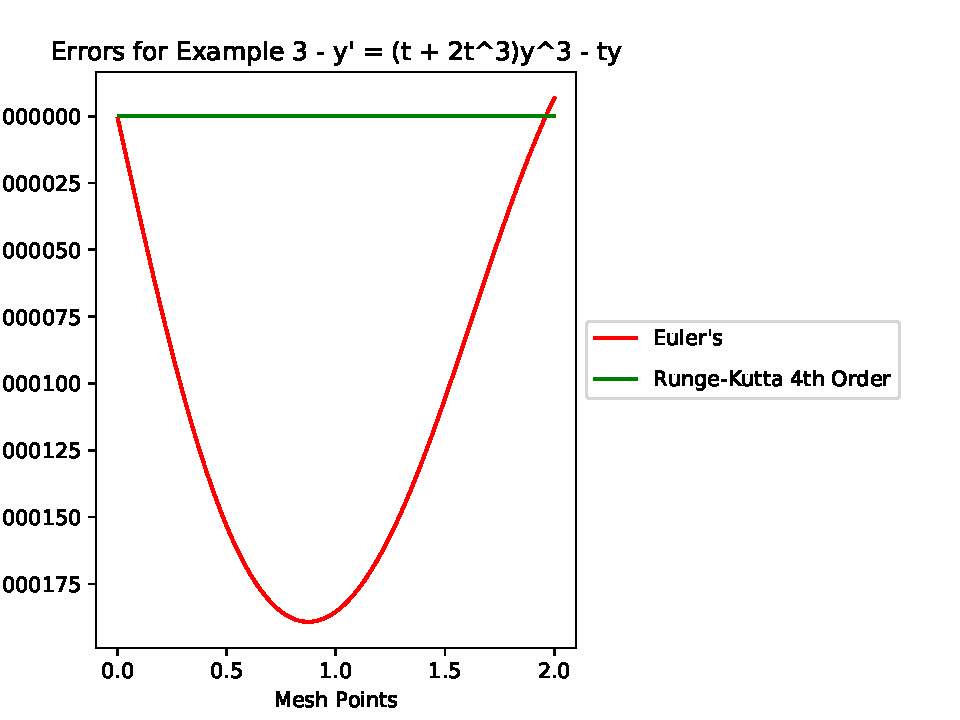
\includegraphics[width=.45\textwidth]{euler_rk4_3}
\caption{Accuracy of Euler vs RK4 when the former has four times smaller step-size. Ex. 3}
\label{fig:euler_rk4_3}
\end{figure}

\begin{figure}[H]
\centering
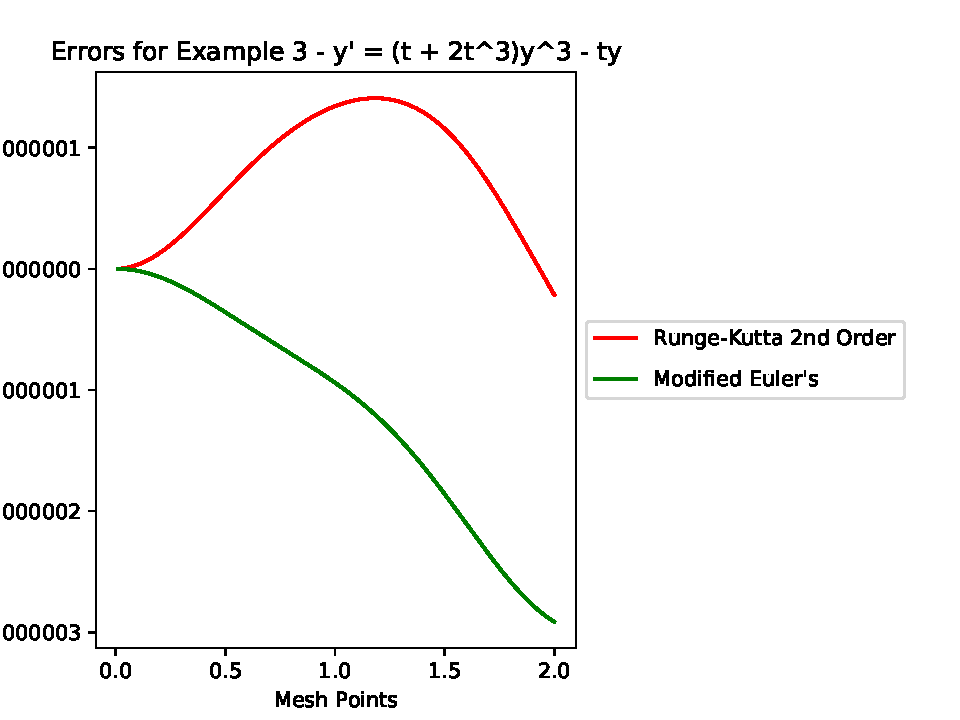
\includegraphics[width=.45\textwidth]{rk2_meuler_3}
\caption{Accuracy of RK2 vs. Modified Euler's method. Ex. 3}
\label{fig:rk2_meuler_3}
\end{figure}

\begin{figure}[H]
\centering
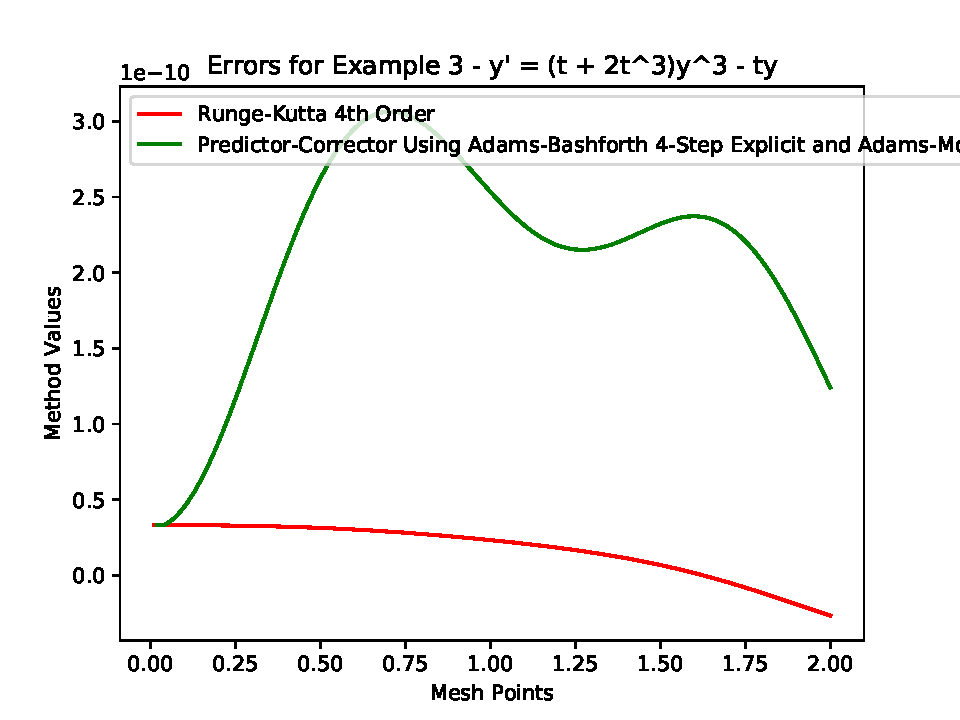
\includegraphics[width=.45\textwidth]{rk4_predictor_3}
\caption{Accuracy of RK4 vs. Adams 4th-order Predictor-Corrector method. Ex. 3}
\label{fig:rk4_predictor_3}
\end{figure}
\clearpage
\section{Discussion}

\subsection{Performance after step-size adjusted for number of evaluations}
methods with local truncation error of higher order seem to perform better even after the step size has been adjusted for number of evaluations. 
This is due to the exponential growing faster than multiplication

\subsection{RK2 vs Modified Euler}
The summary of what error tables reveal and why one may be better than the other

\subsection{RK4 vs PC(mainly)}
Which one does better based on error tables. Advantages of one over
the other depending on situation 
%This is a major part for this project. It should constitute your findings and thoughts. 
%Based on the tests you have,
%you want to comment on the performance of these methods and how would you
%suggest to use in practice. Have extensive discussions with your team members
%and give detailed reasonings for your claims. You can cite books, papers, or other
%resources, such as \cite{Burden:2011a}. ``References'' part below should show
%(only) those you cited in the main paper.


\section{Summary}
%A quick summary to conclude the term paper using a paragraph or two.
test 

\bibliographystyle{abbrv}
\bibliography{my_references}

\end{document}

